% Options for packages loaded elsewhere
\PassOptionsToPackage{unicode}{hyperref}
\PassOptionsToPackage{hyphens}{url}
\PassOptionsToPackage{dvipsnames,svgnames,x11names}{xcolor}
%
\documentclass[
  xelatex,
  ja=standard]{bxjsarticle}

\usepackage{amsmath,amssymb}
\usepackage{iftex}
\ifPDFTeX
  \usepackage[T1]{fontenc}
  \usepackage[utf8]{inputenc}
  \usepackage{textcomp} % provide euro and other symbols
\else % if luatex or xetex
  \usepackage{unicode-math}
  \defaultfontfeatures{Scale=MatchLowercase}
  \defaultfontfeatures[\rmfamily]{Ligatures=TeX,Scale=1}
\fi
\usepackage{lmodern}
\ifPDFTeX\else  
    % xetex/luatex font selection
  \setmainfont[BoldFont=Noto Sans CJK JP]{Noto Serif CJK JP}
\fi
% Use upquote if available, for straight quotes in verbatim environments
\IfFileExists{upquote.sty}{\usepackage{upquote}}{}
\IfFileExists{microtype.sty}{% use microtype if available
  \usepackage[]{microtype}
  \UseMicrotypeSet[protrusion]{basicmath} % disable protrusion for tt fonts
}{}
\makeatletter
\@ifundefined{KOMAClassName}{% if non-KOMA class
  \IfFileExists{parskip.sty}{%
    \usepackage{parskip}
  }{% else
    \setlength{\parindent}{0pt}
    \setlength{\parskip}{6pt plus 2pt minus 1pt}}
}{% if KOMA class
  \KOMAoptions{parskip=half}}
\makeatother
\usepackage{xcolor}
\setlength{\emergencystretch}{3em} % prevent overfull lines
\setcounter{secnumdepth}{5}
% Make \paragraph and \subparagraph free-standing
\ifx\paragraph\undefined\else
  \let\oldparagraph\paragraph
  \renewcommand{\paragraph}[1]{\oldparagraph{#1}\mbox{}}
\fi
\ifx\subparagraph\undefined\else
  \let\oldsubparagraph\subparagraph
  \renewcommand{\subparagraph}[1]{\oldsubparagraph{#1}\mbox{}}
\fi


\providecommand{\tightlist}{%
  \setlength{\itemsep}{0pt}\setlength{\parskip}{0pt}}\usepackage{longtable,booktabs,array}
\usepackage{calc} % for calculating minipage widths
% Correct order of tables after \paragraph or \subparagraph
\usepackage{etoolbox}
\makeatletter
\patchcmd\longtable{\par}{\if@noskipsec\mbox{}\fi\par}{}{}
\makeatother
% Allow footnotes in longtable head/foot
\IfFileExists{footnotehyper.sty}{\usepackage{footnotehyper}}{\usepackage{footnote}}
\makesavenoteenv{longtable}
\usepackage{graphicx}
\makeatletter
\def\maxwidth{\ifdim\Gin@nat@width>\linewidth\linewidth\else\Gin@nat@width\fi}
\def\maxheight{\ifdim\Gin@nat@height>\textheight\textheight\else\Gin@nat@height\fi}
\makeatother
% Scale images if necessary, so that they will not overflow the page
% margins by default, and it is still possible to overwrite the defaults
% using explicit options in \includegraphics[width, height, ...]{}
\setkeys{Gin}{width=\maxwidth,height=\maxheight,keepaspectratio}
% Set default figure placement to htbp
\makeatletter
\def\fps@figure{htbp}
\makeatother

\renewcommand{\thefootnote}{\arabic{footnote}}
\makeatletter
\@ifpackageloaded{tcolorbox}{}{\usepackage[skins,breakable]{tcolorbox}}
\@ifpackageloaded{fontawesome5}{}{\usepackage{fontawesome5}}
\definecolor{quarto-callout-color}{HTML}{909090}
\definecolor{quarto-callout-note-color}{HTML}{0758E5}
\definecolor{quarto-callout-important-color}{HTML}{CC1914}
\definecolor{quarto-callout-warning-color}{HTML}{EB9113}
\definecolor{quarto-callout-tip-color}{HTML}{00A047}
\definecolor{quarto-callout-caution-color}{HTML}{FC5300}
\definecolor{quarto-callout-color-frame}{HTML}{acacac}
\definecolor{quarto-callout-note-color-frame}{HTML}{4582ec}
\definecolor{quarto-callout-important-color-frame}{HTML}{d9534f}
\definecolor{quarto-callout-warning-color-frame}{HTML}{f0ad4e}
\definecolor{quarto-callout-tip-color-frame}{HTML}{02b875}
\definecolor{quarto-callout-caution-color-frame}{HTML}{fd7e14}
\makeatother
\makeatletter
\makeatother
\makeatletter
\makeatother
\makeatletter
\@ifpackageloaded{caption}{}{\usepackage{caption}}
\AtBeginDocument{%
\ifdefined\contentsname
  \renewcommand*\contentsname{目次}
\else
  \newcommand\contentsname{目次}
\fi
\ifdefined\listfigurename
  \renewcommand*\listfigurename{図一覧}
\else
  \newcommand\listfigurename{図一覧}
\fi
\ifdefined\listtablename
  \renewcommand*\listtablename{表一覧}
\else
  \newcommand\listtablename{表一覧}
\fi
\ifdefined\figurename
  \renewcommand*\figurename{図}
\else
  \newcommand\figurename{図}
\fi
\ifdefined\tablename
  \renewcommand*\tablename{表}
\else
  \newcommand\tablename{表}
\fi
}
\@ifpackageloaded{float}{}{\usepackage{float}}
\floatstyle{ruled}
\@ifundefined{c@chapter}{\newfloat{codelisting}{h}{lop}}{\newfloat{codelisting}{h}{lop}[chapter]}
\floatname{codelisting}{コード}
\newcommand*\listoflistings{\listof{codelisting}{コード一覧}}
\makeatother
\makeatletter
\@ifpackageloaded{caption}{}{\usepackage{caption}}
\@ifpackageloaded{subcaption}{}{\usepackage{subcaption}}
\makeatother
\makeatletter
\@ifpackageloaded{tcolorbox}{}{\usepackage[skins,breakable]{tcolorbox}}
\makeatother
\makeatletter
\@ifundefined{shadecolor}{\definecolor{shadecolor}{rgb}{.97, .97, .97}}
\makeatother
\makeatletter
\makeatother
\makeatletter
\makeatother
\ifLuaTeX
\usepackage[bidi=basic]{babel}
\else
\usepackage[bidi=default]{babel}
\fi
\babelprovide[main,import]{japanese}
% get rid of language-specific shorthands (see #6817):
\let\LanguageShortHands\languageshorthands
\def\languageshorthands#1{}
\ifLuaTeX
  \usepackage{selnolig}  % disable illegal ligatures
\fi
\usepackage[]{natbib}
\bibliographystyle{jecon}
\IfFileExists{bookmark.sty}{\usepackage{bookmark}}{\usepackage{hyperref}}
\IfFileExists{xurl.sty}{\usepackage{xurl}}{} % add URL line breaks if available
\urlstyle{same} % disable monospaced font for URLs
\hypersetup{
  pdftitle={政策効果の検証:基礎},
  pdfauthor={土井翔平},
  pdflang={ja},
  colorlinks=true,
  linkcolor={NavyBlue},
  filecolor={Maroon},
  citecolor={NavyBlue},
  urlcolor={NavyBlue},
  pdfcreator={LaTeX via pandoc}}

\title{政策効果の検証:基礎}
\usepackage{etoolbox}
\makeatletter
\providecommand{\subtitle}[1]{% add subtitle to \maketitle
  \apptocmd{\@title}{\par {\large #1 \par}}{}{}
}
\makeatother
\subtitle{技術政策学(データ科学編)}
\author{土井翔平}
\date{2023-05-29}

\begin{document}
\maketitle
\ifdefined\Shaded\renewenvironment{Shaded}{\begin{tcolorbox}[enhanced, interior hidden, sharp corners, borderline west={3pt}{0pt}{shadecolor}, boxrule=0pt, breakable, frame hidden]}{\end{tcolorbox}}\fi

\hypertarget{ux306fux3058ux3081ux306b}{%
\section*{はじめに}\label{ux306fux3058ux3081ux306b}}
\addcontentsline{toc}{section}{はじめに}

近年、\href{https://www.cao.go.jp/others/kichou/ebpm/ebpm.html}{\textbf{証拠に基づく政策立案}}
(evidence-based policy making: EBPM) の重要性が主張されている。

\begin{itemize}
\tightlist
\item
  行政官の経験や勘に頼らない意思決定
\item
  policy-based evidence makingの回避
\item
  \href{https://trends.google.co.jp/trends/explore?date=today\%205-y\&geo=JP\&q=EBPM\&hl=ja}{Google
  Trendsの傾向}
\end{itemize}

\(\leadsto\)証拠とはなにか?

\begin{enumerate}
\def\labelenumi{\arabic{enumi}.}
\tightlist
\item
  政策の効果:ある政策によってどの程度、目標のアウトカムは変化したのか?

  \begin{itemize}
  \tightlist
  \item
    政策効果と\href{https://www.soumu.go.jp/main_sosiki/hyouka/seisaku_n/portal/index.html}{政策評価}とは似て非なるもの。
  \item
    政策評価:目標をどの程度、実現したのか?
  \item
    例:訪日観光客\(n\)万人という目標の実現と、観光政策によって訪日観光客がどの程度増えたのかは別
  \end{itemize}
\item
  \href{https://www.digital.go.jp/assets/contents/node/basic_page/field_ref_resources/5535bc46-b873-42a7-99d6-bb0b70e2470d/20211104_meeting_EBPM_17.pdf}{ロジックモデル}:政策資源の投入から政策成果までの論理的繋がりを可視化し、KPIを定めたもの。

  \begin{itemize}
  \tightlist
  \item
    あくまで、論理を可視化するもので、それ自体が証拠ではない。
  \end{itemize}
\end{enumerate}

\(\leadsto\)この授業では証拠=政策効果として議論する。

\begin{tcolorbox}[enhanced jigsaw, colbacktitle=quarto-callout-warning-color!10!white, arc=.35mm, breakable, title=\textcolor{quarto-callout-warning-color}{\faExclamationTriangle}\hspace{0.5em}{警告}, toprule=.15mm, coltitle=black, bottomrule=.15mm, colframe=quarto-callout-warning-color-frame, leftrule=.75mm, bottomtitle=1mm, opacityback=0, toptitle=1mm, titlerule=0mm, rightrule=.15mm, left=2mm, opacitybacktitle=0.6, colback=white]

講師は政策評価の専門家ではないので、他の授業(例えば、政策評価論や行政学系のもの)では異なる説明があると思われる。どちらが正しいというものではないことに留意。

\end{tcolorbox}

\begin{itemize}
\tightlist
\item
  \href{https://cyberagentailab.github.io/EBPMDB/}{統計的因果推論の例}
\item
  統計的\textbf{因果推論} (statistical causal
  inference):原因と結果の関係(効果)を統計的に分析する

  \begin{itemize}
  \tightlist
  \item
    マーケティングなどでも役に立つ
  \item
    事例研究をするときにも(データを使わなくても)役に立つ(かも)
  \end{itemize}
\end{itemize}

\hypertarget{ux4ea4ux7d61}{%
\section{交絡}\label{ux4ea4ux7d61}}

\hypertarget{ux30efux30afux30c1ux30f3ux306eux52b9ux679c}{%
\subsection{ワクチンの効果}\label{ux30efux30afux30c1ux30f3ux306eux52b9ux679c}}

\textbf{データ=証拠ではない!}

\begin{itemize}
\tightlist
\item
  \href{https://www.covid-datascience.com/post/israeli-data-how-can-efficacy-vs-severe-disease-be-strong-when-60-of-hospitalized-are-vaccinated}{新型コロナワクチンを例に}
\end{itemize}

ワクチン接種者の方が重症者 (sever cases) が多い?

\begin{figure}[htpb]

{\centering 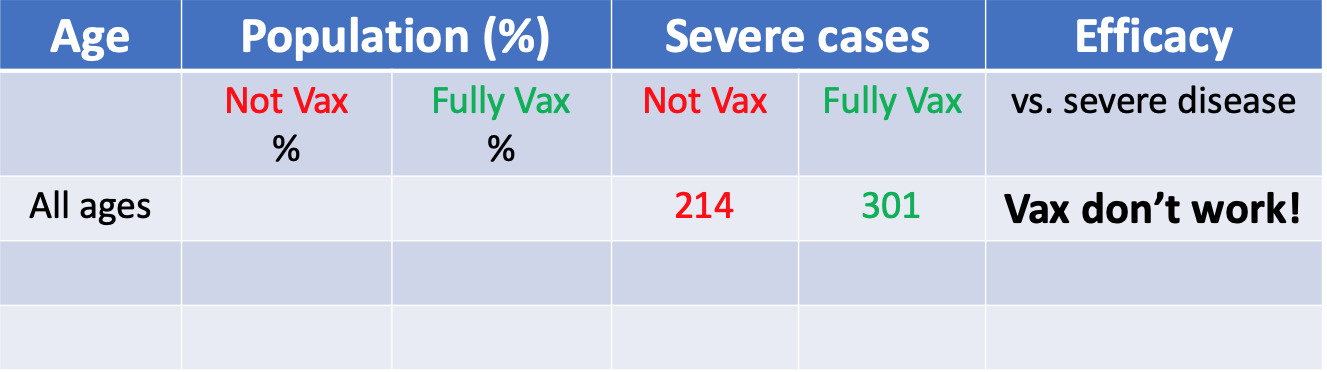
\includegraphics{figures/covid1.png}

}

\caption{Israeli data: How can efficacy vs.~severe disease be strong
when 60\% of hospitalized are vaccinated?}

\end{figure}

\(67.5%
\)の人はワクチンを打っていれば重症化しなかった?

\begin{figure}[htpb]

{\centering 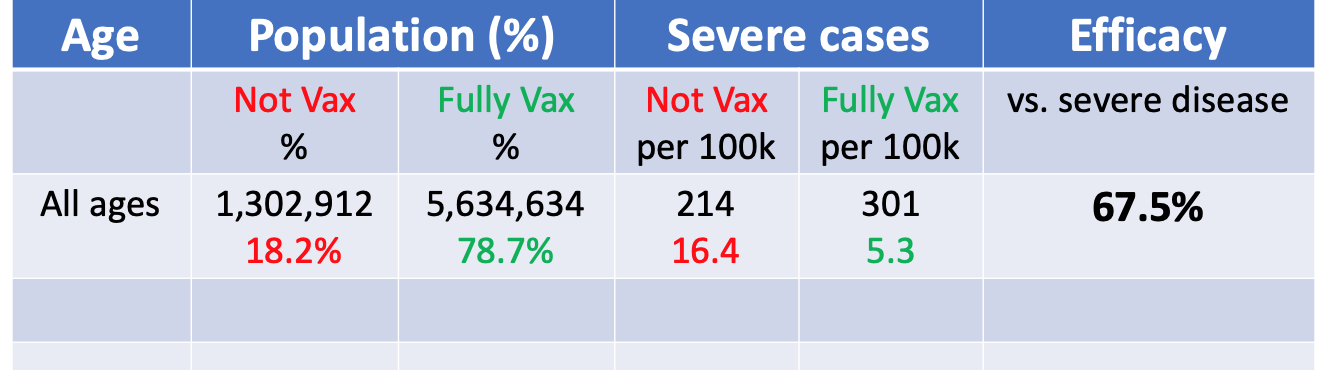
\includegraphics{figures/covid2.png}

}

\caption{Israeli data: How can efficacy vs.~severe disease be strong
when 60\% of hospitalized are vaccinated?}

\end{figure}

\begin{itemize}
\tightlist
\item
  有効性:\((16.4 - 5.3)/16.4 \approx 67.5\%\)
\end{itemize}

世代で分けると有効性が変わる?

\begin{figure}[htpb]

{\centering 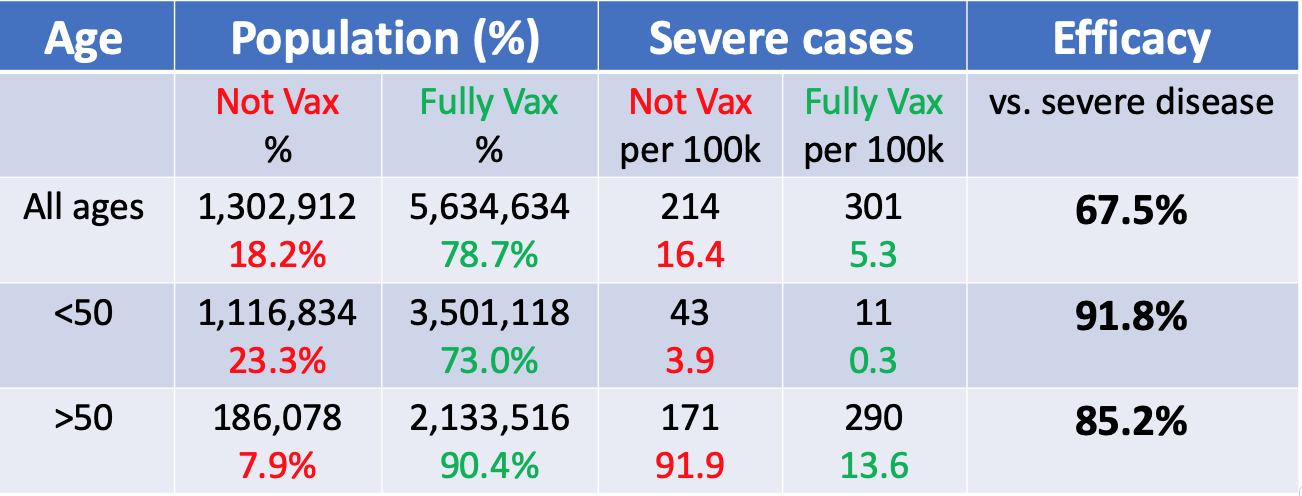
\includegraphics{figures/covid3.png}

}

\caption{Israeli data: How can efficacy vs.~severe disease be strong
when 60\% of hospitalized are vaccinated?}

\end{figure}

ワクチンを接種するかどうかは(パンデミック初期は)重症化のしやすさに影響を受けていた。

\begin{figure}[htpb]

{\centering 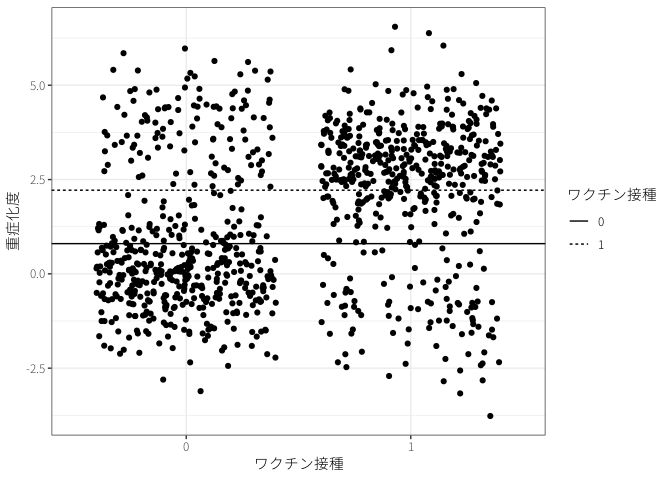
\includegraphics{causal_inference_basic_files/figure-pdf/unnamed-chunk-2-1.png}

}

\caption{ワクチン接種と重症化の架空の例}

\end{figure}

\begin{figure}[htpb]

{\centering 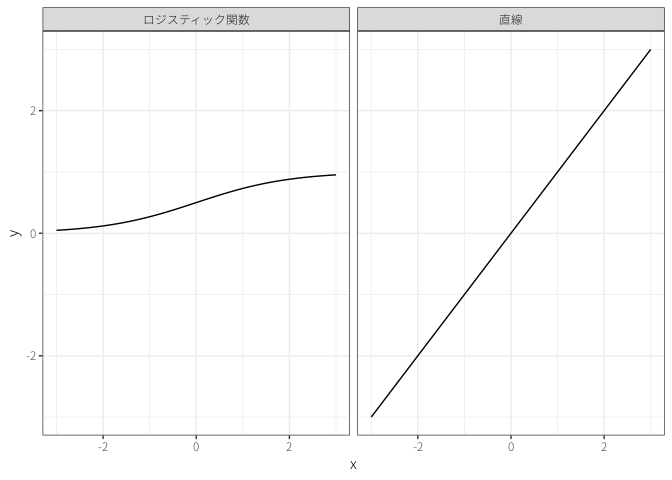
\includegraphics{causal_inference_basic_files/figure-pdf/unnamed-chunk-3-1.png}

}

\caption{ワクチン接種と重症化の架空の例}

\end{figure}

\(\leadsto\)原因(政策)の有無で結果の違いが生じていても、効果とは言えない!

\hypertarget{ux4ea4ux7d61-1}{%
\subsection{交絡}\label{ux4ea4ux7d61-1}}

なぜ、単純な比較をするだけでは正しく効果を計算できなかったのか?

\textbf{交絡}
(confounding):原因と関係し、結果にも影響するような第三の要因がある状況

\begin{itemize}
\tightlist
\item
  そのような要因を交絡因子 (confounder) や共変量 (covariate) と呼ぶ。
\end{itemize}

\begin{figure}[htpb]

{\centering 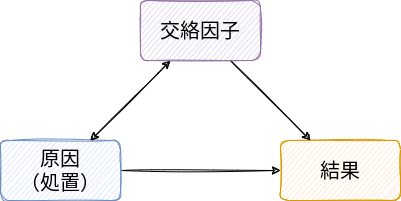
\includegraphics{figures/confounding1.drawio.png}

}

\caption{交絡の可視化}

\end{figure}

\begin{itemize}
\tightlist
\item
  原因→結果の関係を知りたいけれど、原因↔交絡因子→結果の関係(バックドアパス)があるので、正確に分析できない。
\item
  因果関係ではないけれど相関関係が生じていることを見かけの相関 (spurious
  correlation) と呼ぶ。\footnote{本来は\href{https://www.tylervigen.com/spurious-correlations}{無関係なものが相関している}状況を指していた。}

  \begin{itemize}
  \tightlist
  \item
    相関関係は因果関係の前提と言われることがあるが、そうではない点に注意。
  \end{itemize}
\end{itemize}

どのような交絡の例があるだろうか?

\(\leadsto\)交絡を取り除かない限り、データから効果を示すことはできない。

\begin{itemize}
\tightlist
\item
  事例分析をする際も同様

  \begin{itemize}
  \tightlist
  \item
    ある政策を行った自治体とそうではない自治体
  \item
    ある自治体がある政策を行う前と後
  \end{itemize}
\end{itemize}

\hypertarget{ux30e9ux30f3ux30c0ux30e0ux5316ux6bd4ux8f03ux8a66ux9a13}{%
\section{ランダム化比較試験}\label{ux30e9ux30f3ux30c0ux30e0ux5316ux6bd4ux8f03ux8a66ux9a13}}

理想:全く同じ人がワクチンを受けた場合と受けなかった場合に重症化するかどうかを比較する。

\(\leadsto\)不可能

現実:同じような集団がワクチンを受けた場合と受けなかった場合に重症化するかどうかを比較する。

\(\leadsto\)どのようにして「同じような集団」を作るのか?

シンプルかつ強力な方法としての\textbf{ランダム化比較試験} (randomized
controlled trial: RCT)

\begin{itemize}
\tightlist
\item
  RCT:対象をランダムに分割して、一方には原因を与え、他方には原因を与えず、集団の結果を比較する。
\end{itemize}

\begin{figure}[htpb]

{\centering 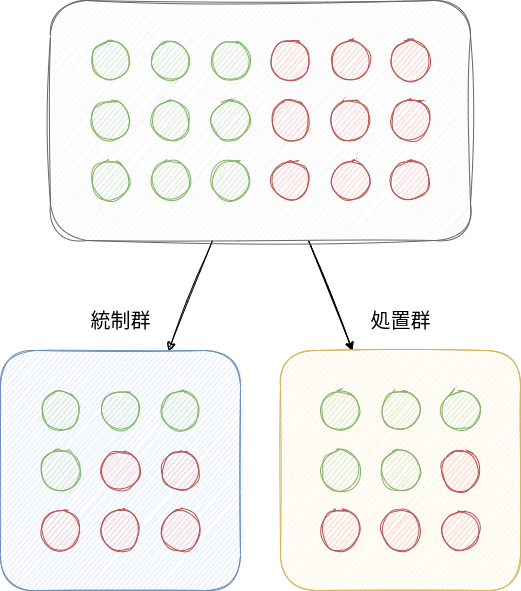
\includegraphics{figures/randomization.drawio.png}

}

\caption{RCTのイメージ}

\end{figure}

RCTで交絡(バックドア・パス)を消す!

\begin{itemize}
\tightlist
\item
  ランダムにワクチンを摂取すれば年齢などとは無関係なはず。
\end{itemize}

\begin{figure}[htpb]

{\centering 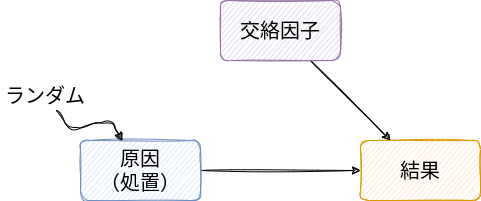
\includegraphics{figures/confounding2.drawio.png}

}

\caption{RCTの可視化}

\end{figure}

\hypertarget{ux30d5ux30a3ux30fcux30ebux30c9ux5b9fux9a13}{%
\subsection{フィールド実験}\label{ux30d5ux30a3ux30fcux30ebux30c9ux5b9fux9a13}}

フィールド実験:現実世界にランダムに介入して、\textbf{実際の行動}の変化を分析

\begin{itemize}
\tightlist
\item
  A/Bテストを初めとするオンラインテスト
\item
  実際に政策をランダムに試行する。
\end{itemize}

開発経済学を中心にRCTが活用\citep{banerjee2012, leigh2020}

\begin{itemize}
\tightlist
\item
  貧困層が移住しないのは資金が足りないからなのか、情報が足りないからなのか?\citep{bryan2014}
\end{itemize}

\begin{figure}[htpb]

{\centering 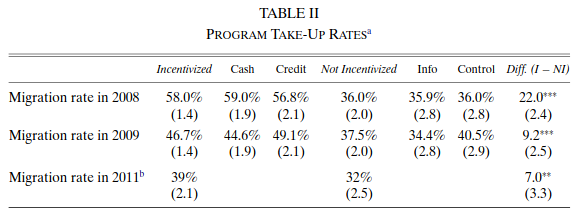
\includegraphics{figures/bryan.png}

}

\caption{\citet{bryan2014}}

\end{figure}

\begin{itemize}
\tightlist
\item
  中等教育は経済的に豊かになるのか?\citep{duflo2021}
\end{itemize}

\begin{figure}[htpb]

{\centering 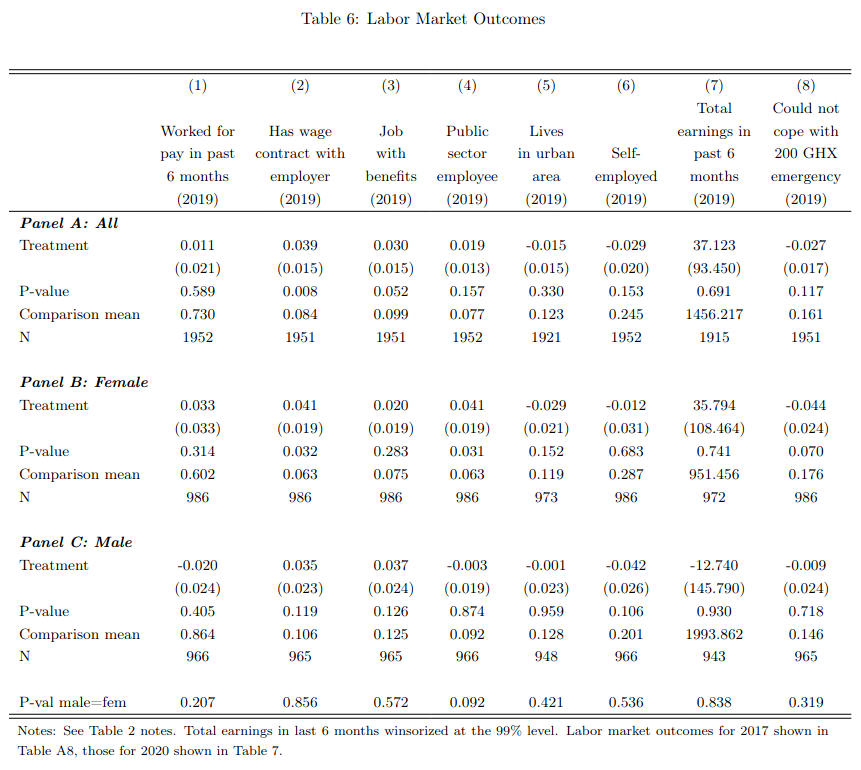
\includegraphics{figures/duflo.png}

}

\caption{\citet{duflo2021}}

\end{figure}

\begin{itemize}
\tightlist
\item
  どのようなメッセージだと人々は投票へ行くのか?\citep{gerber2008}
\end{itemize}

\begin{figure}[htpb]

{\centering 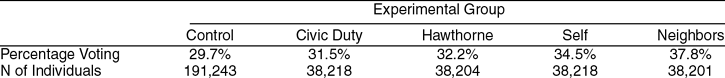
\includegraphics{figures/gerber.png}

}

\caption{\citet{gerber2008}}

\end{figure}

\hypertarget{ux30b5ux30fcux30d9ux30a4ux5b9fux9a13}{%
\subsection{サーベイ実験}\label{ux30b5ux30fcux30d9ux30a4ux5b9fux9a13}}

サーベイ実験:世論調査(サーベイ)にランダムな項目を入れ、\textbf{表明された意見}の変化を分析\citep{song2020}

サーベイ実験は政治学や社会学を中心に利用

\begin{itemize}
\tightlist
\item
  人々は移民に関する事実を知ると寛容になるのか?\citep{alesina2023, barrera2020}

  \begin{itemize}
  \tightlist
  \item
    人々は移民の割合などを過大に評価している。
  \end{itemize}
\end{itemize}

\begin{figure}[htpb]

{\centering 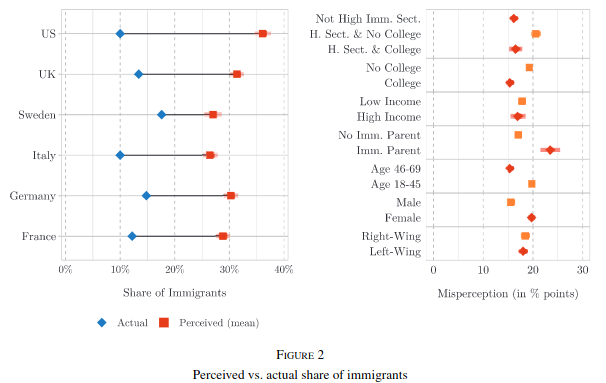
\includegraphics{figures/alesina1.png}

}

\caption{\citet{alesina2023}}

\end{figure}

\begin{itemize}
\tightlist
\item
  移民の事実に関する質問と再配分政策への意見に関する質問の順番をランダムにする。

  \begin{itemize}
  \tightlist
  \item
    移民の事実に関する誤解に気づいた人は再配分に寛容になる?
  \end{itemize}
\end{itemize}

\begin{figure}[htpb]

{\centering 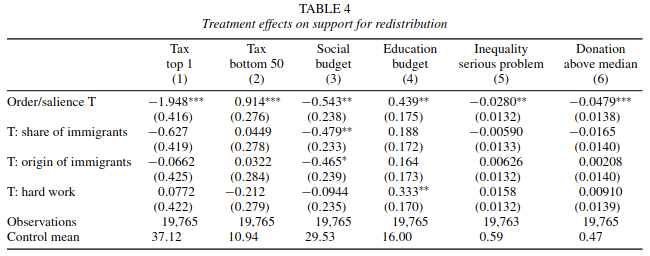
\includegraphics{figures/alesina2.png}

}

\caption{\citet{alesina2023}}

\end{figure}

\begin{itemize}
\tightlist
\item
  移民に関する情報を以下のうちから1つだけランダムに提示し、マリーヌ・ル・ペンへの支持を調査
\end{itemize}

\begin{enumerate}
\def\labelenumi{\arabic{enumi}.}
\tightlist
\item
  なにも示さない
\item
  マリーヌ・ル・ペンの主張(事実ではない)
\item
  事実
\item
  2と3の両方
\end{enumerate}

\begin{figure}[htpb]

{\centering 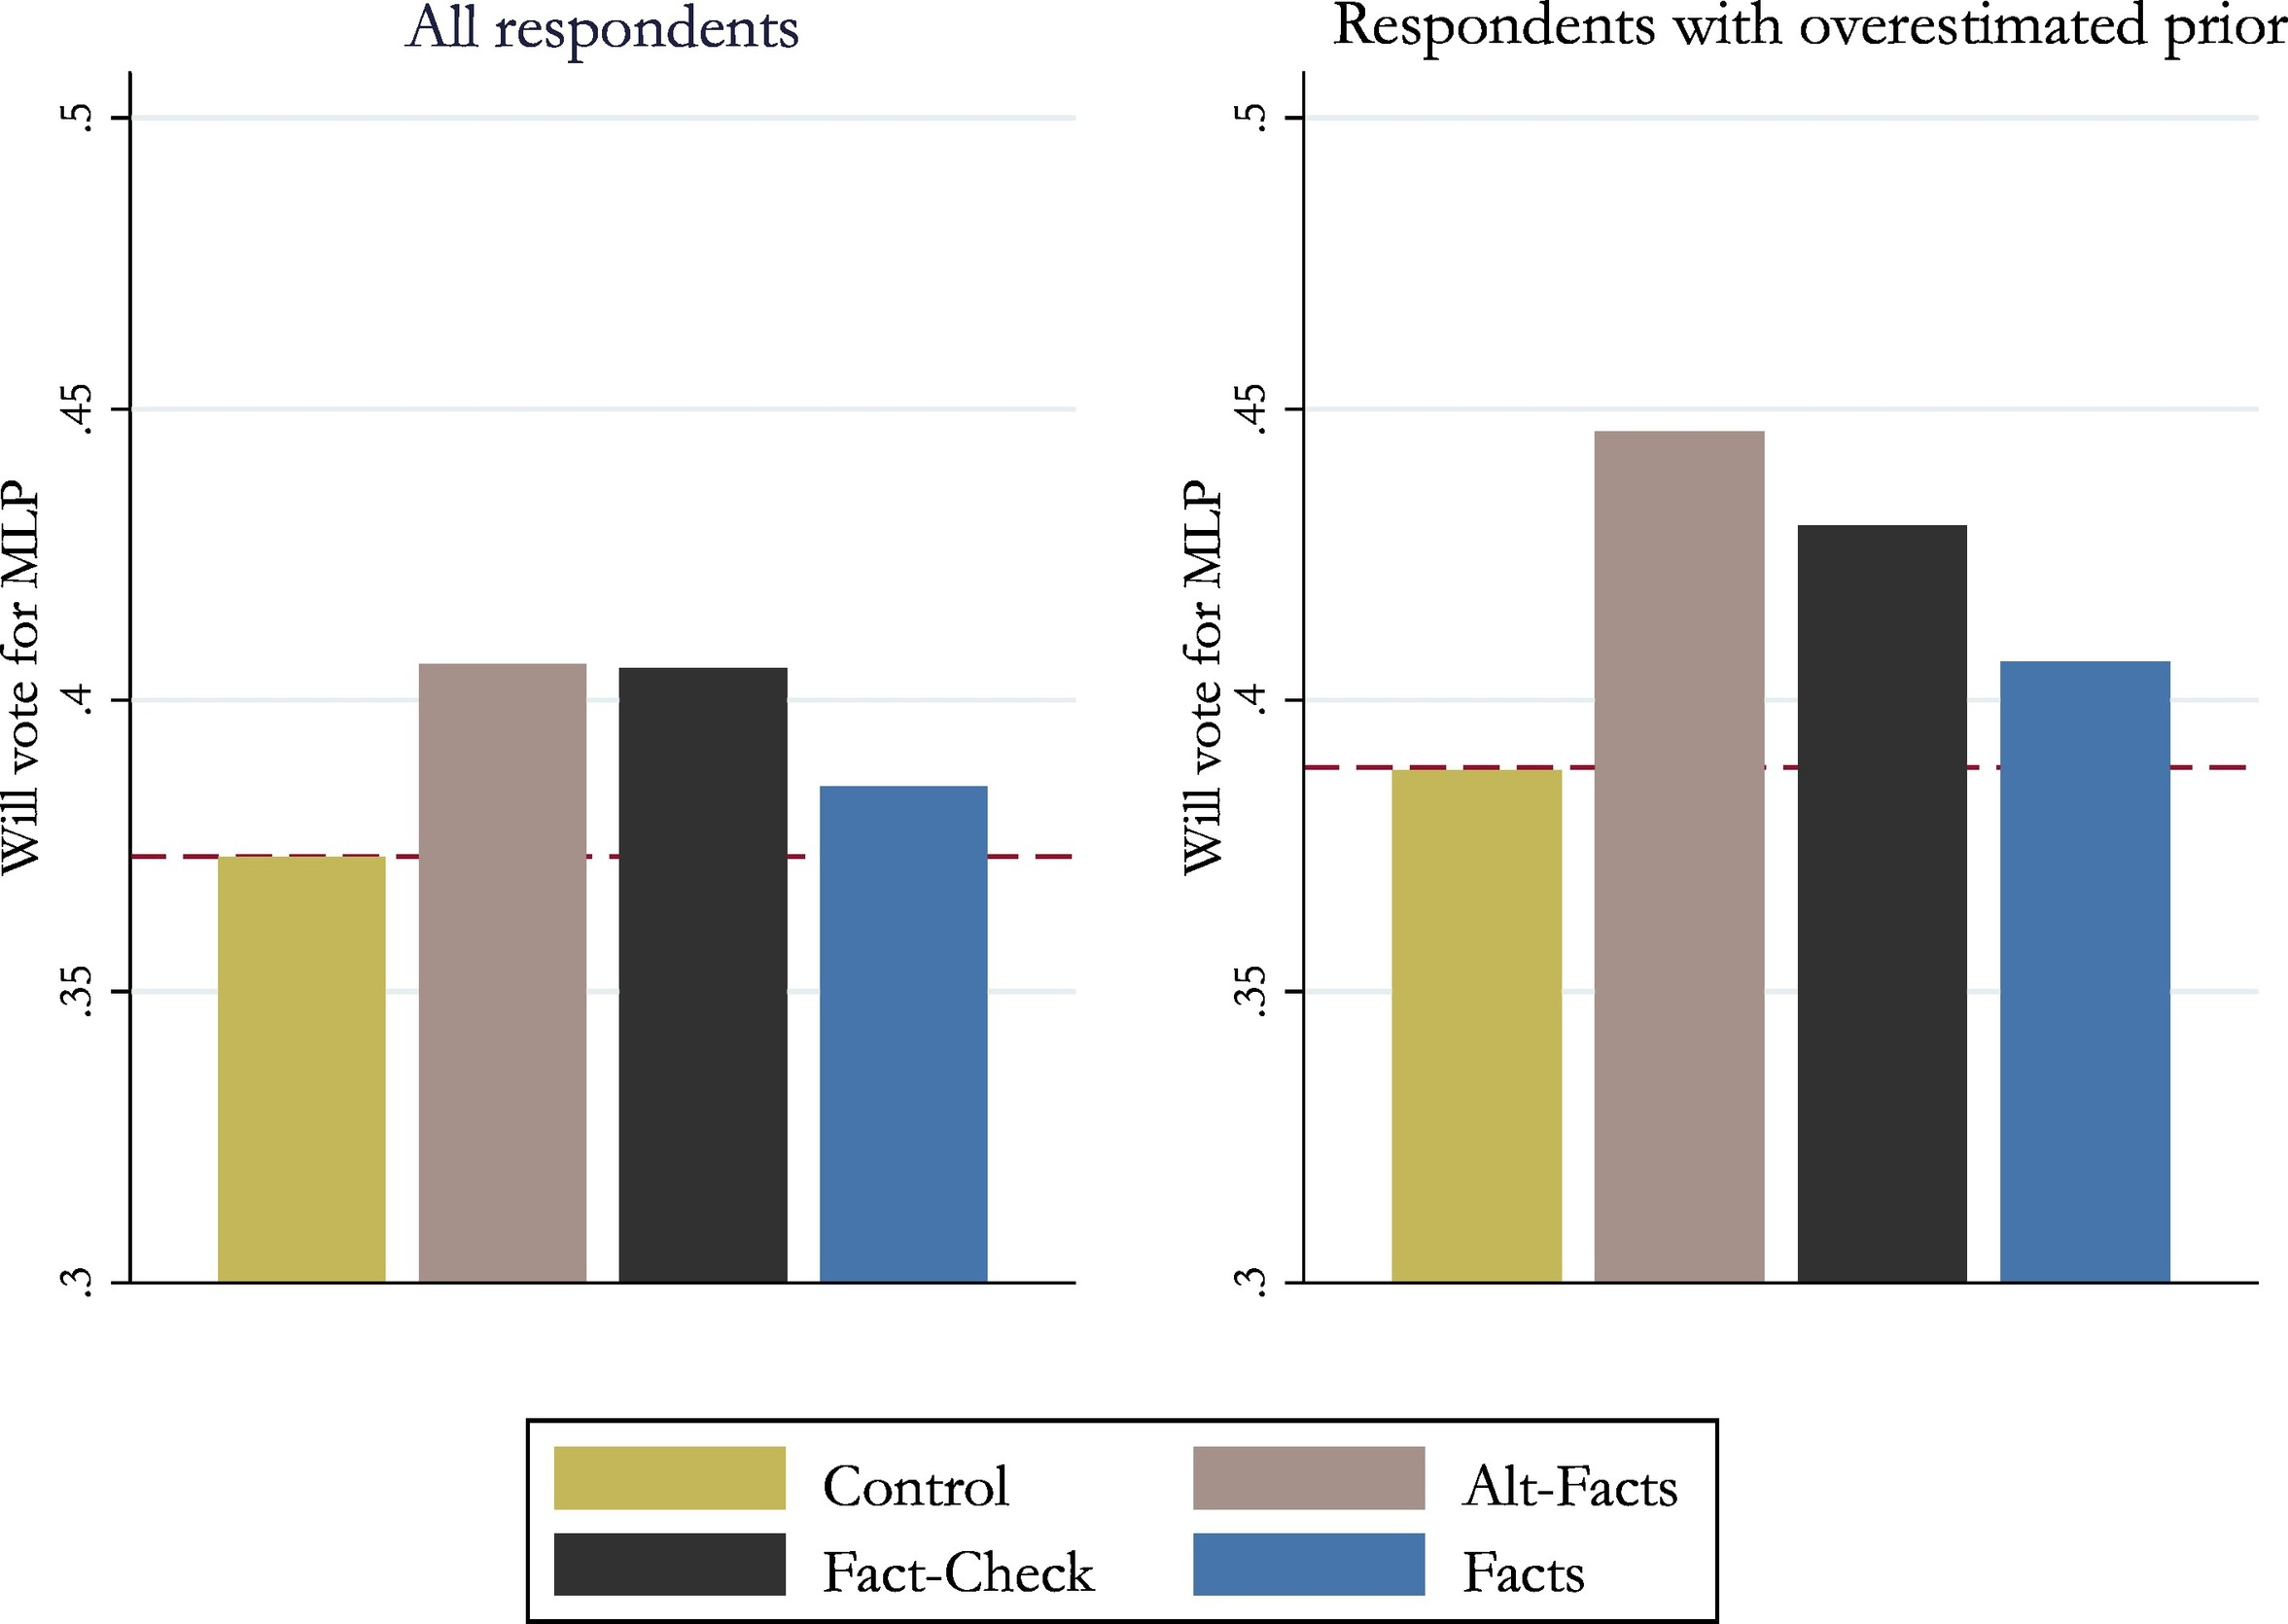
\includegraphics{figures/barrera.jpg}

}

\caption{\citet{barrera2020}}

\end{figure}

\hypertarget{ux30b3ux30f3ux30b8ux30e7ux30a4ux30f3ux30c8ux5b9fux9a13}{%
\subsubsection{コンジョイント実験}\label{ux30b3ux30f3ux30b8ux30e7ux30a4ux30f3ux30c8ux5b9fux9a13}}

コンジョイント実験:2つ(以上)の選択肢を提示し、その要因をランダムに変化させ、どの要因が選択に影響を与えているのかを分析

\begin{itemize}
\tightlist
\item
  人々はどのような政策を重視して投票するのか?

  \begin{itemize}
  \tightlist
  \item
    \href{https://business.nikkei.com/atcl/seminar/19/00059/120200330/}{衆院総選挙、緊急解析! データが明かした有権者の本音}
  \item
    \href{https://business.nikkei.com/atcl/gen/19/00351/120200011/}{マニフェスト選挙を疑え:2021年総選挙の計量政治学}
  \end{itemize}
\end{itemize}

\begin{figure}[htpb]

{\centering 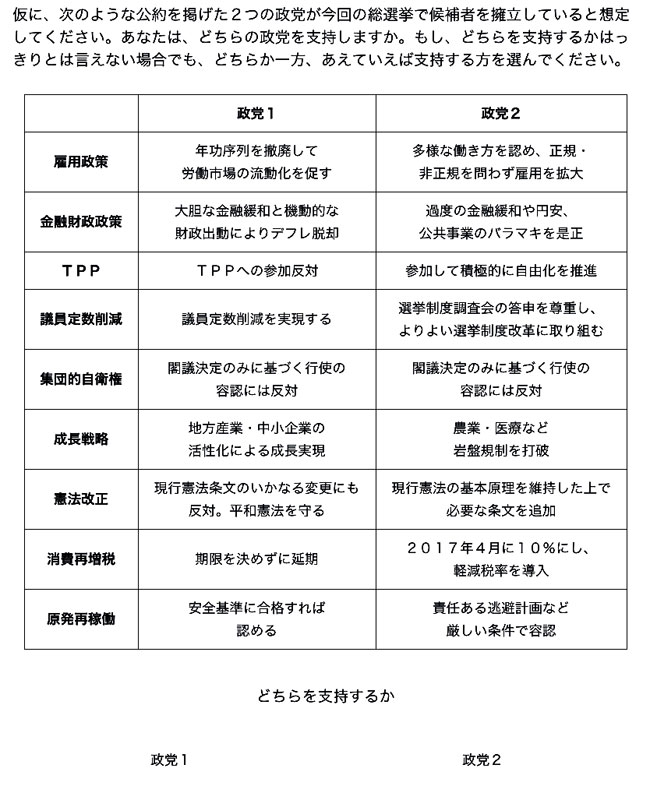
\includegraphics{figures/hyo02.jpg}

}

\caption{コンジョイント分析の例}

\end{figure}

\begin{figure}[htpb]

{\centering 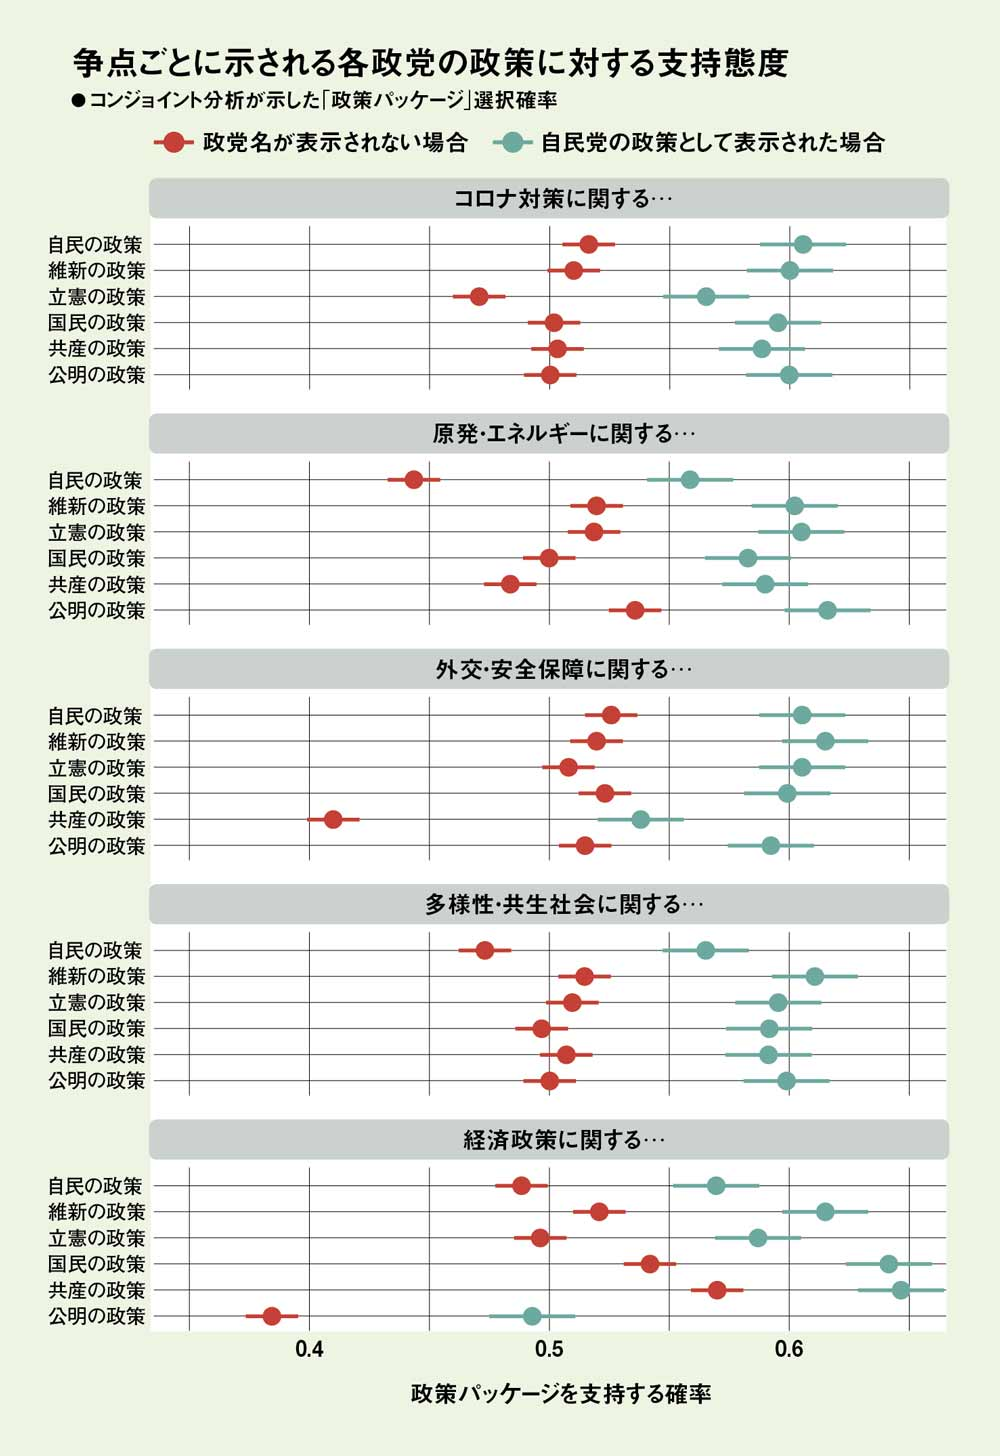
\includegraphics{figures/f3.jpg}

}

\caption{コンジョイント分析の結果}

\end{figure}

\hypertarget{ux30eaux30b9ux30c8ux5b9fux9a13}{%
\subsubsection{リスト実験}\label{ux30eaux30b9ux30c8ux5b9fux9a13}}

\textbf{社会的望ましさバイアス} (social desirebility bias:
SDB):回答者は社会的に望ましい答えをしようとして本音を話さない傾向

リスト実験:該当する項目の数を尋ねることでSDBを回避する実験手法

\begin{itemize}
\tightlist
\item
  人々はどの程度、人種差別をしているのか?\citep{kuklinski1997}
\end{itemize}

\begin{figure}[htpb]

{\centering 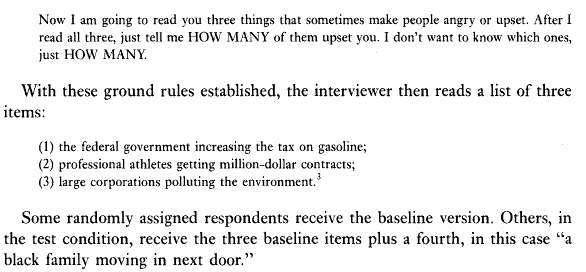
\includegraphics{figures/kuklinski.png}

}

\caption{\citet{kuklinski1997}}

\end{figure}

\begin{itemize}
\tightlist
\item
  知りたい項目が入っているものと、そうでないものをランダムに表示させ、該当数を尋ねる。
\end{itemize}

\hypertarget{ux81eaux7136ux5b9fux9a13}{%
\section{自然実験}\label{ux81eaux7136ux5b9fux9a13}}

\textbf{自然実験} (natural experiment):RCTではないがRCTと同じような状況

\begin{itemize}
\tightlist
\item
  ナショナリズムの高揚は武力紛争に繋がるのか?\citep{bertoli2017}
\end{itemize}

\begin{figure}[htpb]

{\centering 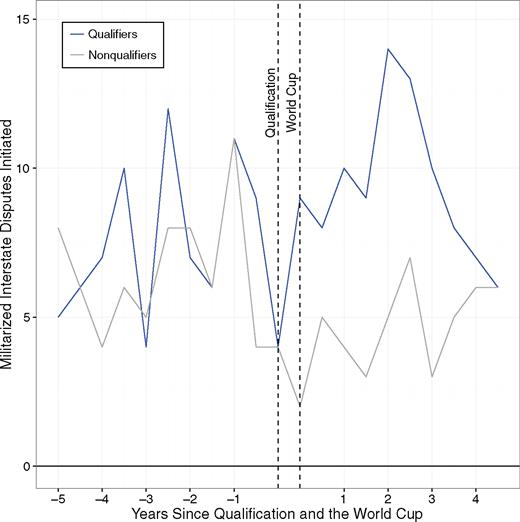
\includegraphics{figures/bertoli.jpeg}

}

\caption{\citet{bertoli2017}}

\end{figure}

\begin{itemize}
\tightlist
\item
  政治的指導者の交代は民主化や平和に繋がるのか?\citep{jones2009}
\end{itemize}

\begin{figure}[htpb]

{\centering 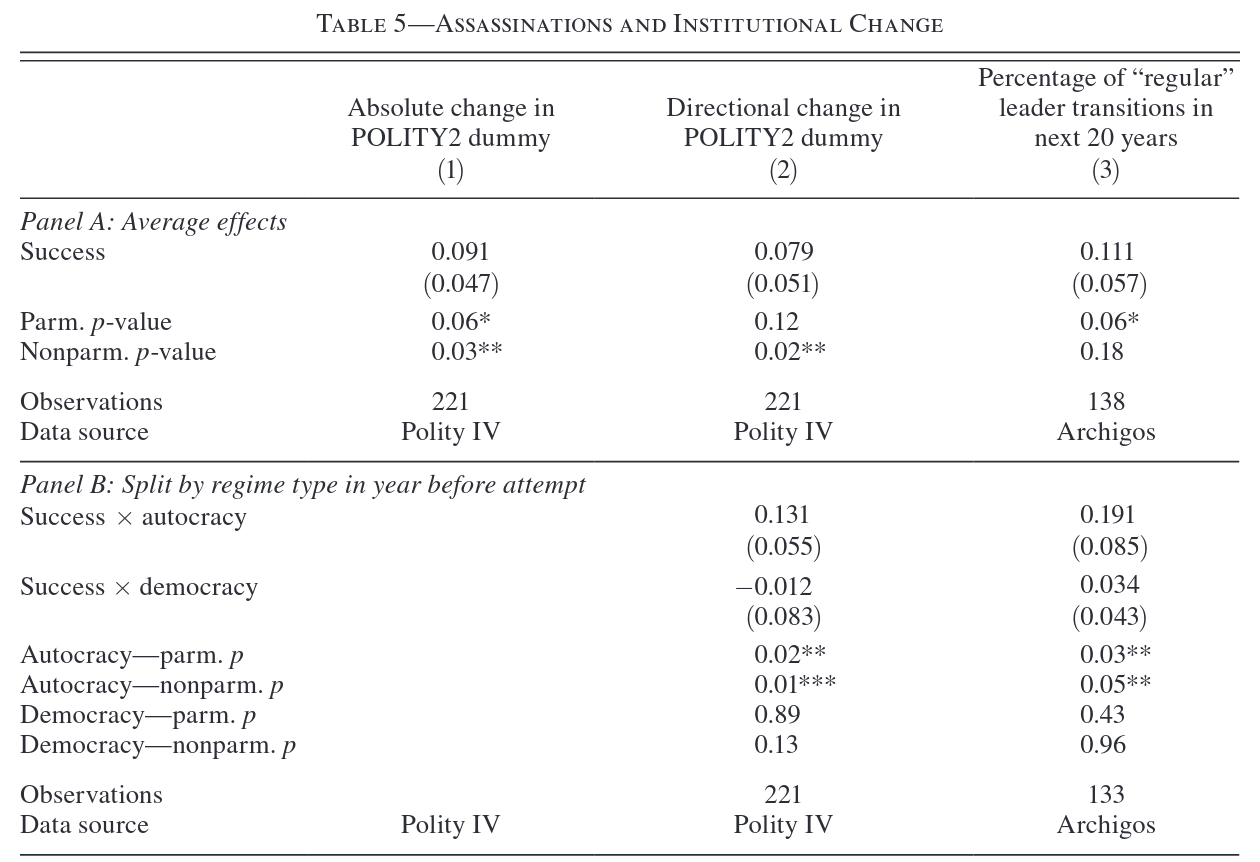
\includegraphics{figures/jones1.png}

}

\caption{\citet{jones2009}}

\end{figure}

\begin{figure}[htpb]

{\centering 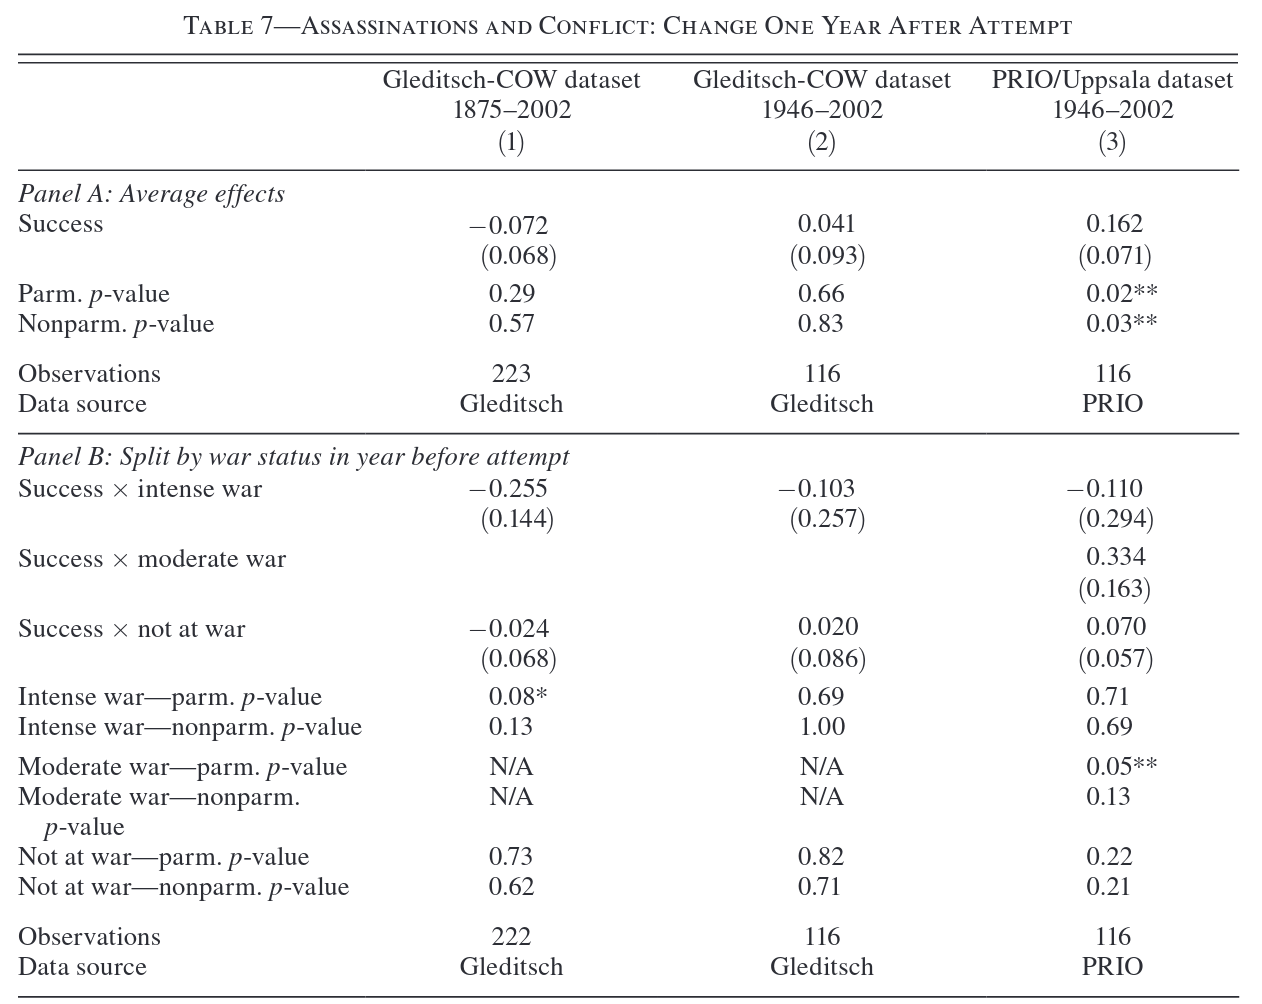
\includegraphics{figures/jones2.png}

}

\caption{\citet{jones2009}}

\end{figure}

\begin{itemize}
\tightlist
\item
  女性医師による治療は死亡率に影響するのか?\citep{tsugawa2017}
\end{itemize}

\begin{figure}[htpb]

{\centering 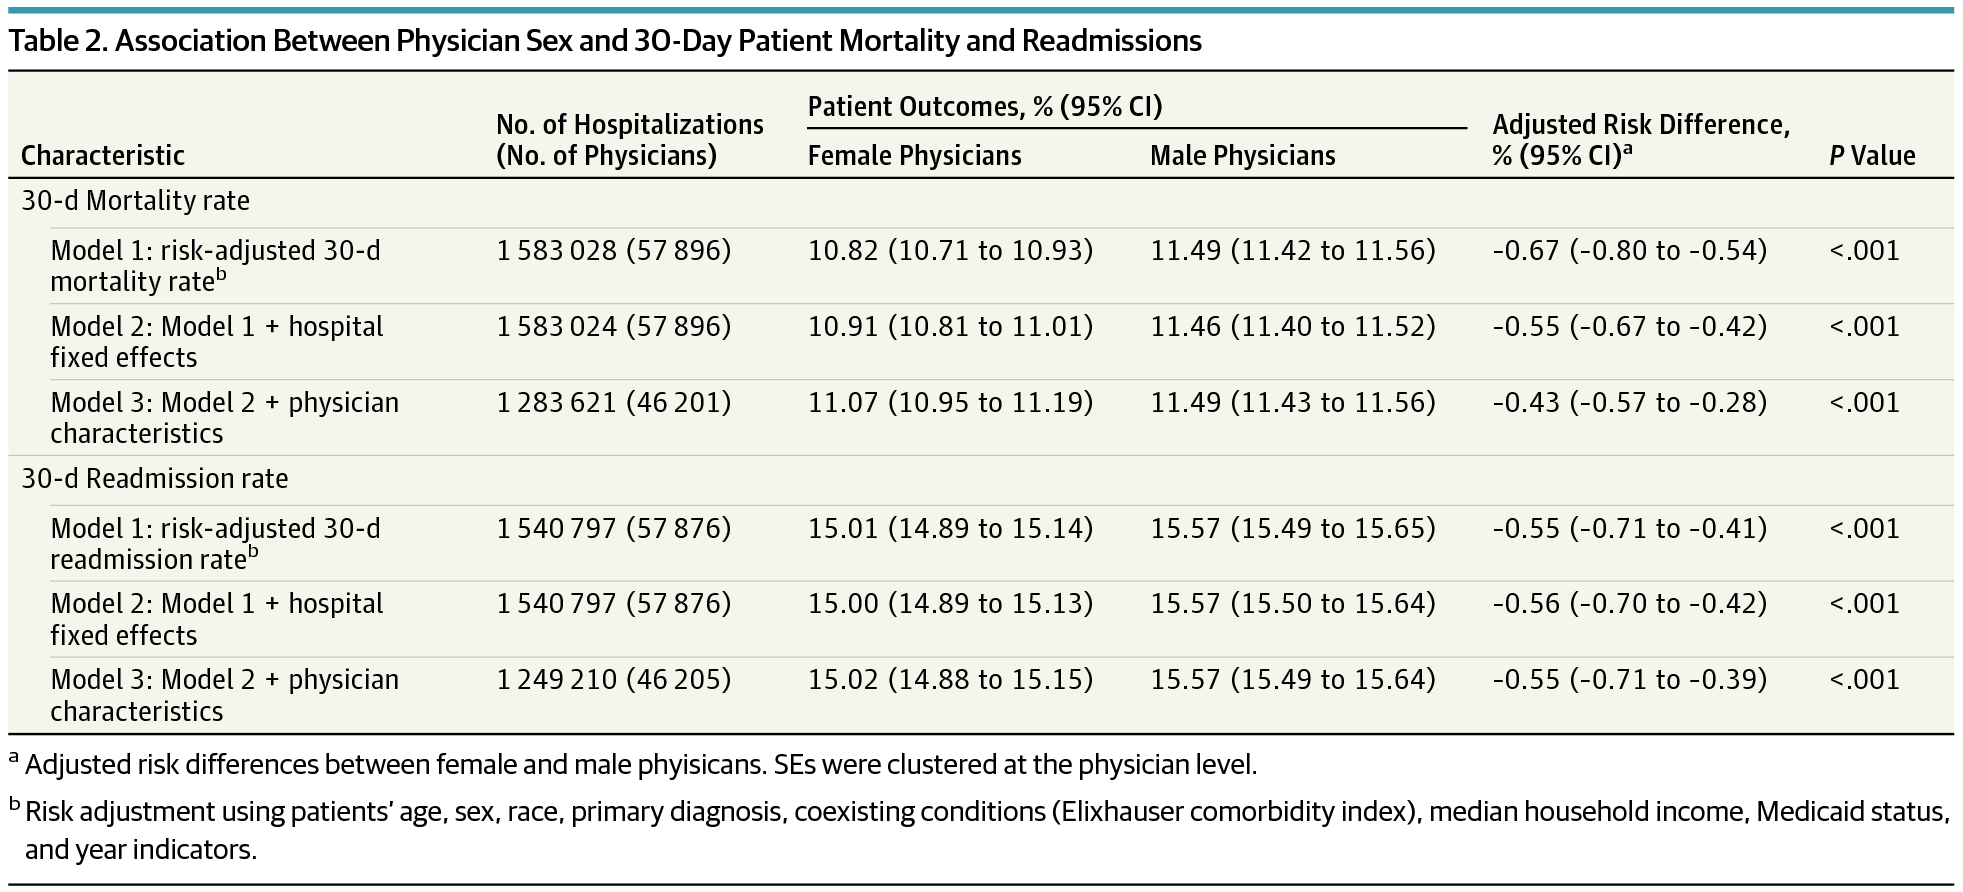
\includegraphics{figures/tsugawa.png}

}

\caption{\citet{tsugawa2017}}

\end{figure}

\hypertarget{ux7d71ux8a08ux7684ux4eeeux8aacux691cux5b9a}{%
\section{統計的仮説検定}\label{ux7d71ux8a08ux7684ux4eeeux8aacux691cux5b9a}}

\begin{tcolorbox}[enhanced jigsaw, colbacktitle=quarto-callout-warning-color!10!white, arc=.35mm, breakable, title=\textcolor{quarto-callout-warning-color}{\faExclamationTriangle}\hspace{0.5em}{警告}, toprule=.15mm, coltitle=black, bottomrule=.15mm, colframe=quarto-callout-warning-color-frame, leftrule=.75mm, bottomtitle=1mm, opacityback=0, toptitle=1mm, titlerule=0mm, rightrule=.15mm, left=2mm, opacitybacktitle=0.6, colback=white]

統計的仮説検定は非常に難しいので、分からなくても構わない。講師を含めてちゃんと理解できているか怪しい。

\end{tcolorbox}

RCTや自然実験であれば、因果効果の大きさは明らかにできる?

\(\leadsto\)偶然、(本来は効果がないはずなのに)2つのグループで差が出てしまった可能性

\textbf{統計的仮説検定}:効果が現れたのが偶然ではないかどうかを判別する方法

\begin{enumerate}
\def\labelenumi{\arabic{enumi}.}
\tightlist
\item
  \textbf{仮に}本当は効果がないとする(帰無仮説: null hypothesis)
\item
  本当は効果がないのに、効果があるように見える実際のデータが生じる確率(p値:
  p-value)を求める。

  \begin{itemize}
  \tightlist
  \item
    p値を求めるときには推定結果の不確実性を表す標準誤差 (standard error:
    SE) を用いる。
  \end{itemize}
\item
  p値が予め設定しておいた値(例えば\(5\%\))を下回っている場合、\textbf{統計的に有意}であると呼ぶ。\footnote{効果の値を標準誤差で割ったものが、およそ\(2\)以上であれば\(5\%\)有意水準で統計的に有意である。}

  \begin{itemize}
  \tightlist
  \item
    本当は効果がないのに\(5\%\)の確率で生じる結果が出たのだとしたら、もはや「効果がない」という前提がおかしいのではないか。
  \end{itemize}
\end{enumerate}

\(\leadsto\)とりあえず、統計的に有意でなければ効果があると強く主張できない。

\begin{enumerate}
\def\labelenumi{\arabic{enumi}.}
\tightlist
\item
  上記の代わりに信頼区間を求めて、信頼区間が0(などの基準点)を含まなかったら統計的に有意であると判断する方法もある。
\end{enumerate}

\begin{figure}[htpb]

{\centering 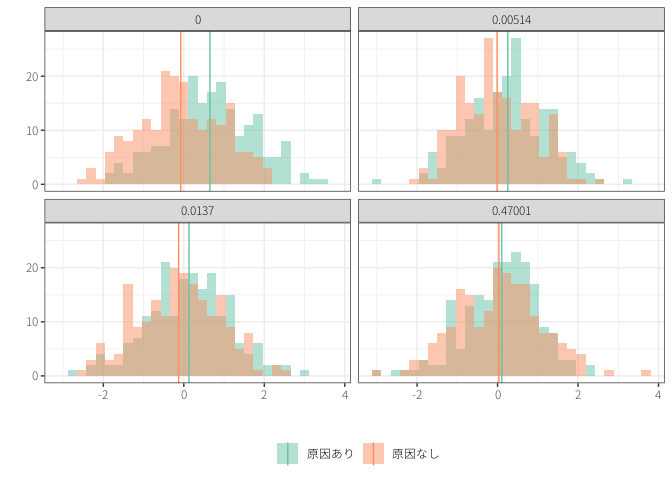
\includegraphics{causal_inference_basic_files/figure-pdf/unnamed-chunk-4-1.png}

}

\end{figure}

\hypertarget{ux8aa4ux89e3ux6ce8ux610fux4e8bux9805}{%
\subsection{誤解・注意事項}\label{ux8aa4ux89e3ux6ce8ux610fux4e8bux9805}}

\begin{enumerate}
\def\labelenumi{\arabic{enumi}.}
\tightlist
\item
  p値が低ければ効果が大きい
\item
  統計的に有意ではないから関係ない
\item
  p値は「効果がない」確率ではない
\end{enumerate}

\hypertarget{ux554fux984cux70b9}{%
\subsection{問題点}\label{ux554fux984cux70b9}}

p値が有意水準以下であるかどうかで二者択一の判断をすることが問題視

\begin{itemize}
\tightlist
\item
  p-hacking:データや分析手法を変えて、統計的有意になるようにする
\item
  出版バイアス:統計的に有意ではない結果 (null result)
  は出版されにくい。
\item
  HARKing (hypothesizing after the results are
  known):データ分析を行い、統計的に有意な結果から仮説を後付けする。
\end{itemize}

\begin{figure}[htpb]

{\centering 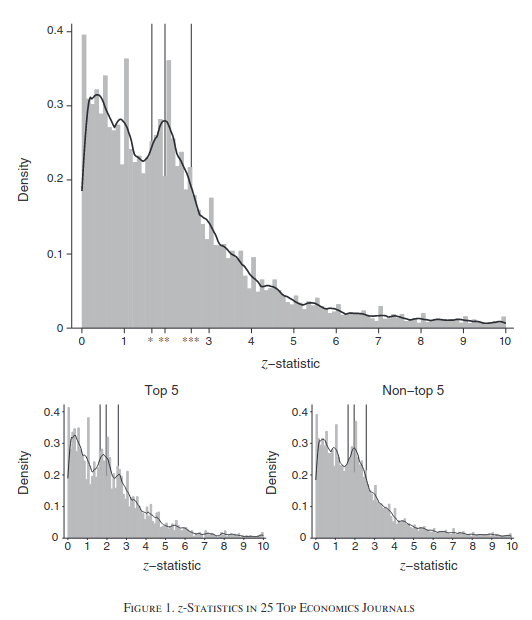
\includegraphics{figures/brodeur.png}

}

\caption{\citet{brodeur2020}}

\end{figure}

\hypertarget{rctux306eux9650ux754cux6ce8ux610fux70b9}{%
\section{RCTの限界・注意点}\label{rctux306eux9650ux754cux6ce8ux610fux70b9}}

交絡がある限り、単純な比較では効果は分からない!

\(\leadsto\)RCTや自然実験のように、同じようなグループを作り出す工夫

\begin{itemize}
\tightlist
\item
  比較事例分析をする場合は、同じようだけど関心のある原因だけは異なるような事例を見つけてくる。
\end{itemize}

\hypertarget{ux30b5ux30f3ux30d7ux30ebux306eux4ee3ux8868ux6027}{%
\subsection{サンプルの代表性}\label{ux30b5ux30f3ux30d7ux30ebux306eux4ee3ux8868ux6027}}

無作為化比較試験:無作為に処置を割り当て\(\leadsto\)効果を推定

\begin{itemize}
\tightlist
\item
  \textbf{内的妥当性} (internal
  validity):手元にあるデータの中で正しく因果推論できる
\end{itemize}

無作為抽出 (random sampling):特定の集団から一部を無作為に取り出すこと

\begin{itemize}
\tightlist
\item
  \textbf{外的妥当性} (external validity)
  :分析結果が分析に用いたデータ以外にも当てはまる

  \begin{itemize}
  \tightlist
  \item
    (サンプルの)代表性:サンプルにおける属性(性別や年齢など)の割合が本当に知りたい集団と似ている。
  \item
    たとえ実験ではなくても世論調査などをする場合は無作為抽出は必要
  \end{itemize}
\end{itemize}

無作為割り当てができていても無作為抽出をしていなければ、分析結果が元々の集団に当てはまるかは分からない。

\begin{itemize}
\tightlist
\item
  手元にあるサンプルにおいて正しく因果推論はできているという意味では間違っていない。
\end{itemize}

\hypertarget{ux4e00ux822cux5747ux8861ux52b9ux679c}{%
\subsection{一般均衡効果}\label{ux4e00ux822cux5747ux8861ux52b9ux679c}}

RCTでは集団全体から一部を取り出して、政策の有無を決定する。

\(\leadsto\)実際に政策を受けるのは全体から見るとごく一部

政策として集団全体に実施した場合は、RCT通りの結果にならないかもしれない。

\(\leadsto\)集団全体における効果(一般均衡効果)が生じる。

\begin{itemize}
\tightlist
\item
  職業訓練や教育が賃金を上げるとしても、全員がプログラムを受けるとその効果は相殺?
\end{itemize}

効果が波及する場合はRCTは適切に政策の効果を推定できない。

\hypertarget{ux5b9fux884cux53efux80fdux6027}{%
\subsection{実行可能性}\label{ux5b9fux884cux53efux80fdux6027}}

RCTや自然実験は因果推論における強力な手法だが、実行可能?

\begin{itemize}
\tightlist
\item
  多くの場合、個人を対象とするミクロな分析

  \begin{itemize}
  \tightlist
  \item
    投票行動や消費者行動とは親和性が高いが、国家の行動や状態を分析することは困難
  \end{itemize}
\item
  処置が倫理的に問題がある可能性\footnote{実験を行う場合は大学の倫理審査委員会で審査を受け、認可される必要がある。}

  \begin{itemize}
  \tightlist
  \item
    嘘の情報や心理的に負担となる情報を与える。
  \item
    資金やトレーニングの提供など一部の人に有利(不利)なものかも
  \end{itemize}
\item
  高額な資金が必要かも

  \begin{itemize}
  \tightlist
  \item
    サーベイ実験の場合、オンラインのクラウドソーシングのサービス\footnote{Yahoo!クラウドソーシング、Amazon
      Mechanical Turk、LUCID Marketplaceなど。}を利用すれば比較的安価に行える。
  \item
    調査会社のサンプルプールを利用する場合は高額
  \item
    フィールド実験の場合は運営費用&現地のパートナーを確保
  \end{itemize}
\item
  (特にサーベイ実験の場合)表明選好に過ぎず、顕示選好ではないかも?

  \begin{itemize}
  \tightlist
  \item
    質問への回答\(\neq\)現実の政治的行動
  \end{itemize}
\item
  都合の良い自然実験はなかなか起こらない。
\end{itemize}

\(\leadsto\)RCTや自然実験以外に政策効果を検証できないか?


  \bibliography{references.bib}


\end{document}
